\chapter{Acercamientos Previos a la Soluci\'on}

\section{Est\'atica: m\'axima ganancia posible}

El sistema tiene una soluci\'on anal\'itica si no existe una restricci\'on en la oferta (es decir, el campo siempre puede cubrir la demanda de la f\'abrica) y cada agente tiene en el d\'ia $n$ informaci\'on acerca de la demanda del d\'ia $n+1$ de su agente inmediatamente inferior. En este caso, los agentes ni siquiera necesitan usar sus almacenes: sencillamente compran cada d\'ia lo necesario para el d\'ia siguiente. Podemos observar el comportamiento de esta soluci\'on en la figura \ref{analytic_1}.

\begin{figure}[ht!]
\caption{Distribuci\'on de Cerveza}
\label{analytic_1}
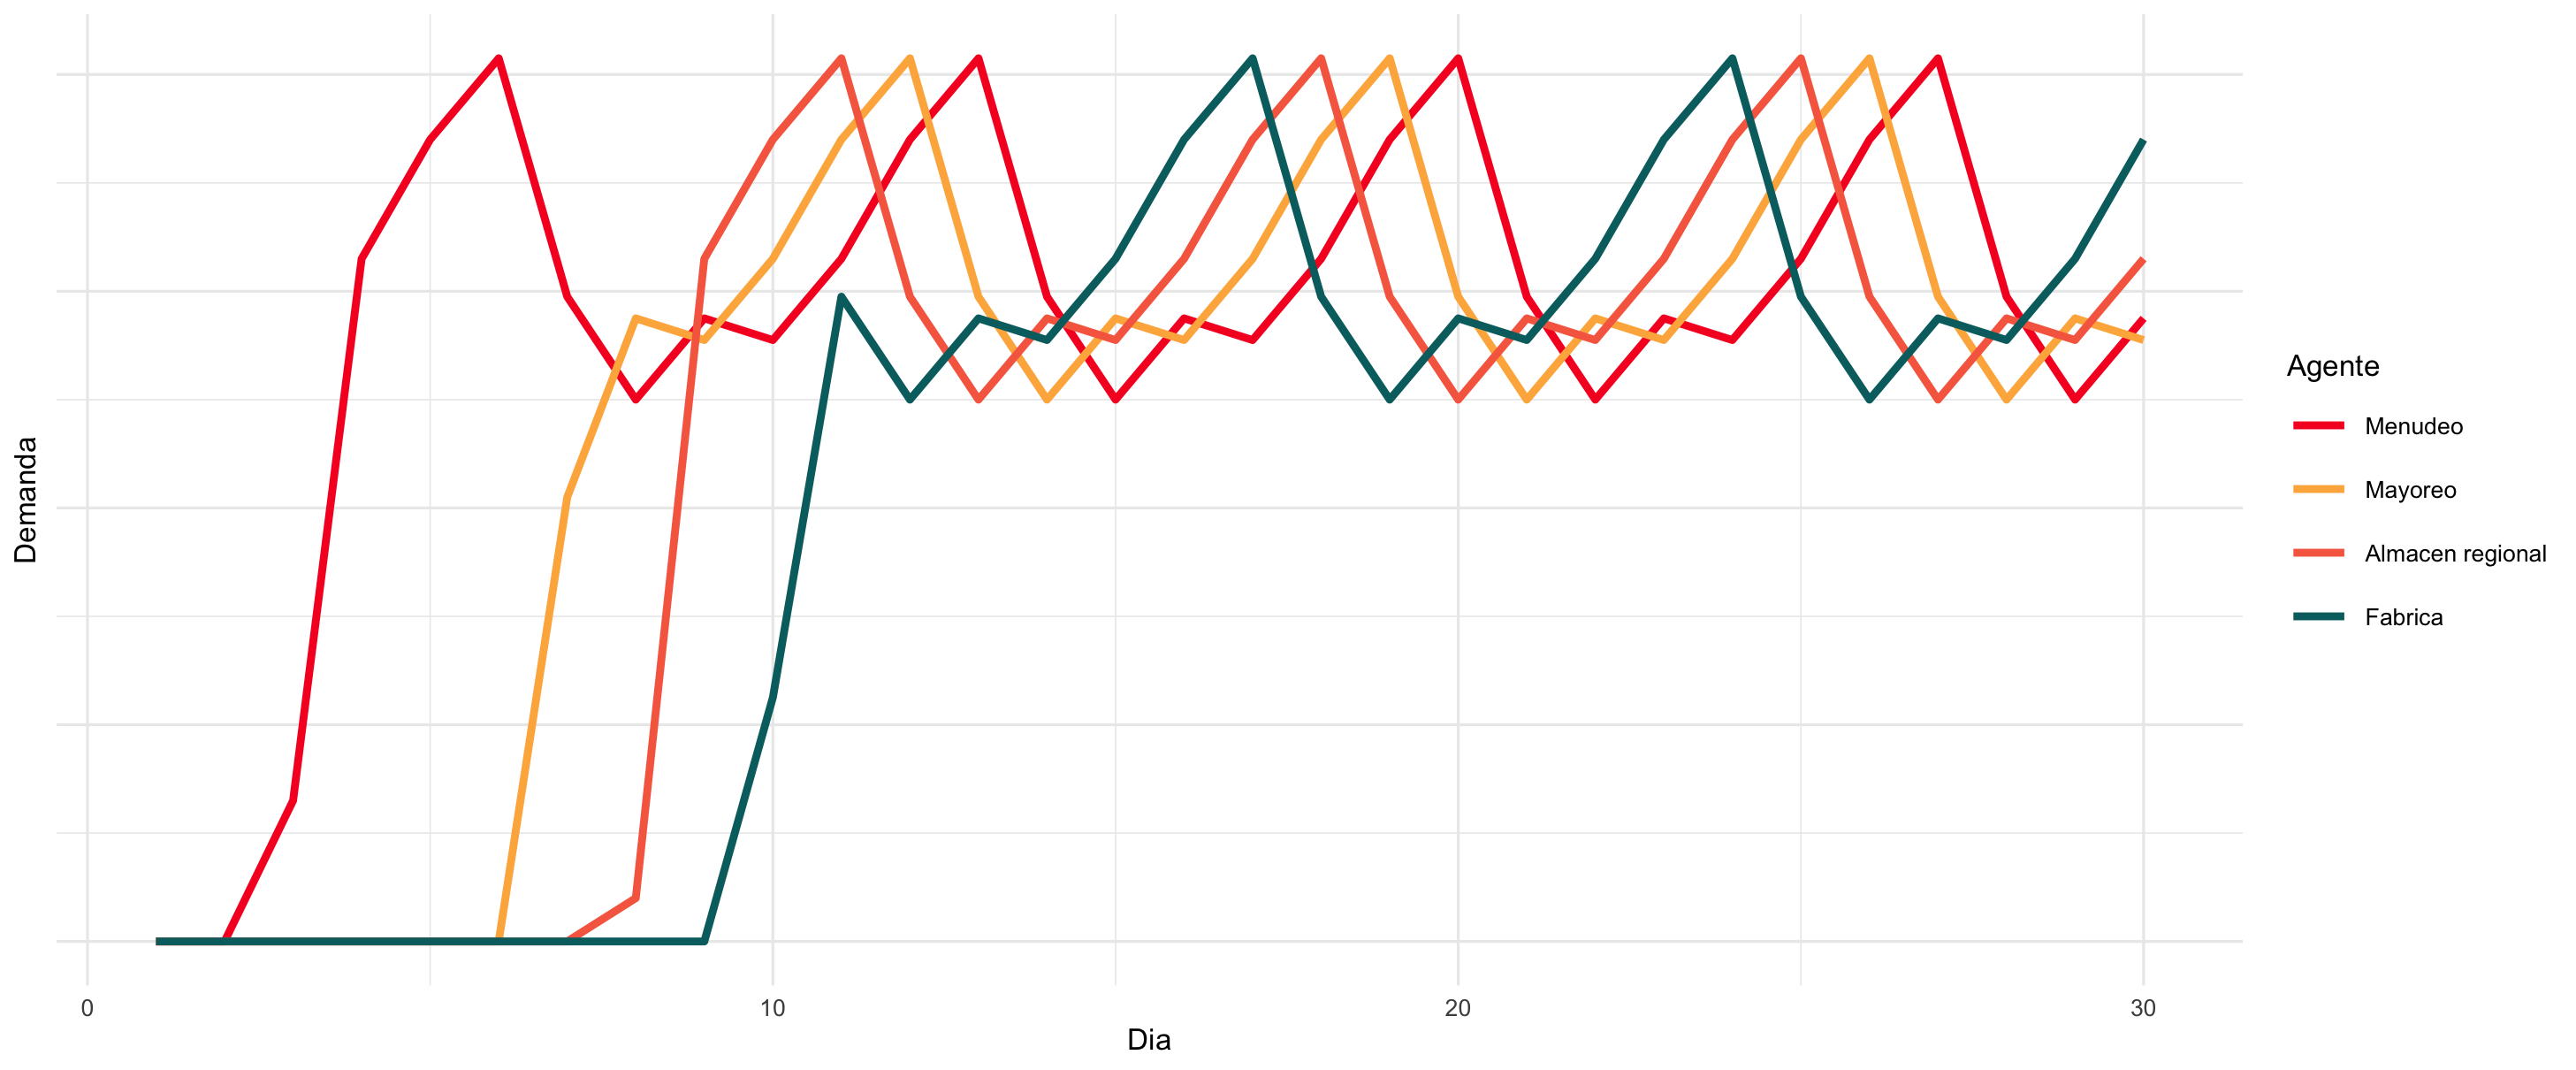
\includegraphics[width=12cm]{tesis_tex/figs/analytic_solution_0_all_0_inv.png}
\centering
\end{figure}

Sin embargo, incluso cuando todos los agentes tienen informaci\'on perfecta, podemos observar una versi\'on muy ligera del efecto l\'atigo. Si el minorista tiene suficiente cerveza para cubrir algunos d\'ias de demanda del consumidor, entonces no tiene incentivo para comprarle al mayorista hasta que su inventario se agote. Esta situaci\'on puede replicarse en los dos niveles superiores, de tal manera que la f\'abrica no recibe nada de informaci\'on acerca de la demanda del consumidor durante una cantidad considerable de tiempo. Este efecto se puede observar en la figura \ref{analytic_2}.

\begin{figure}[ht!]
\caption{Distribuci\'on de Cerveza}
\label{analytic_2}
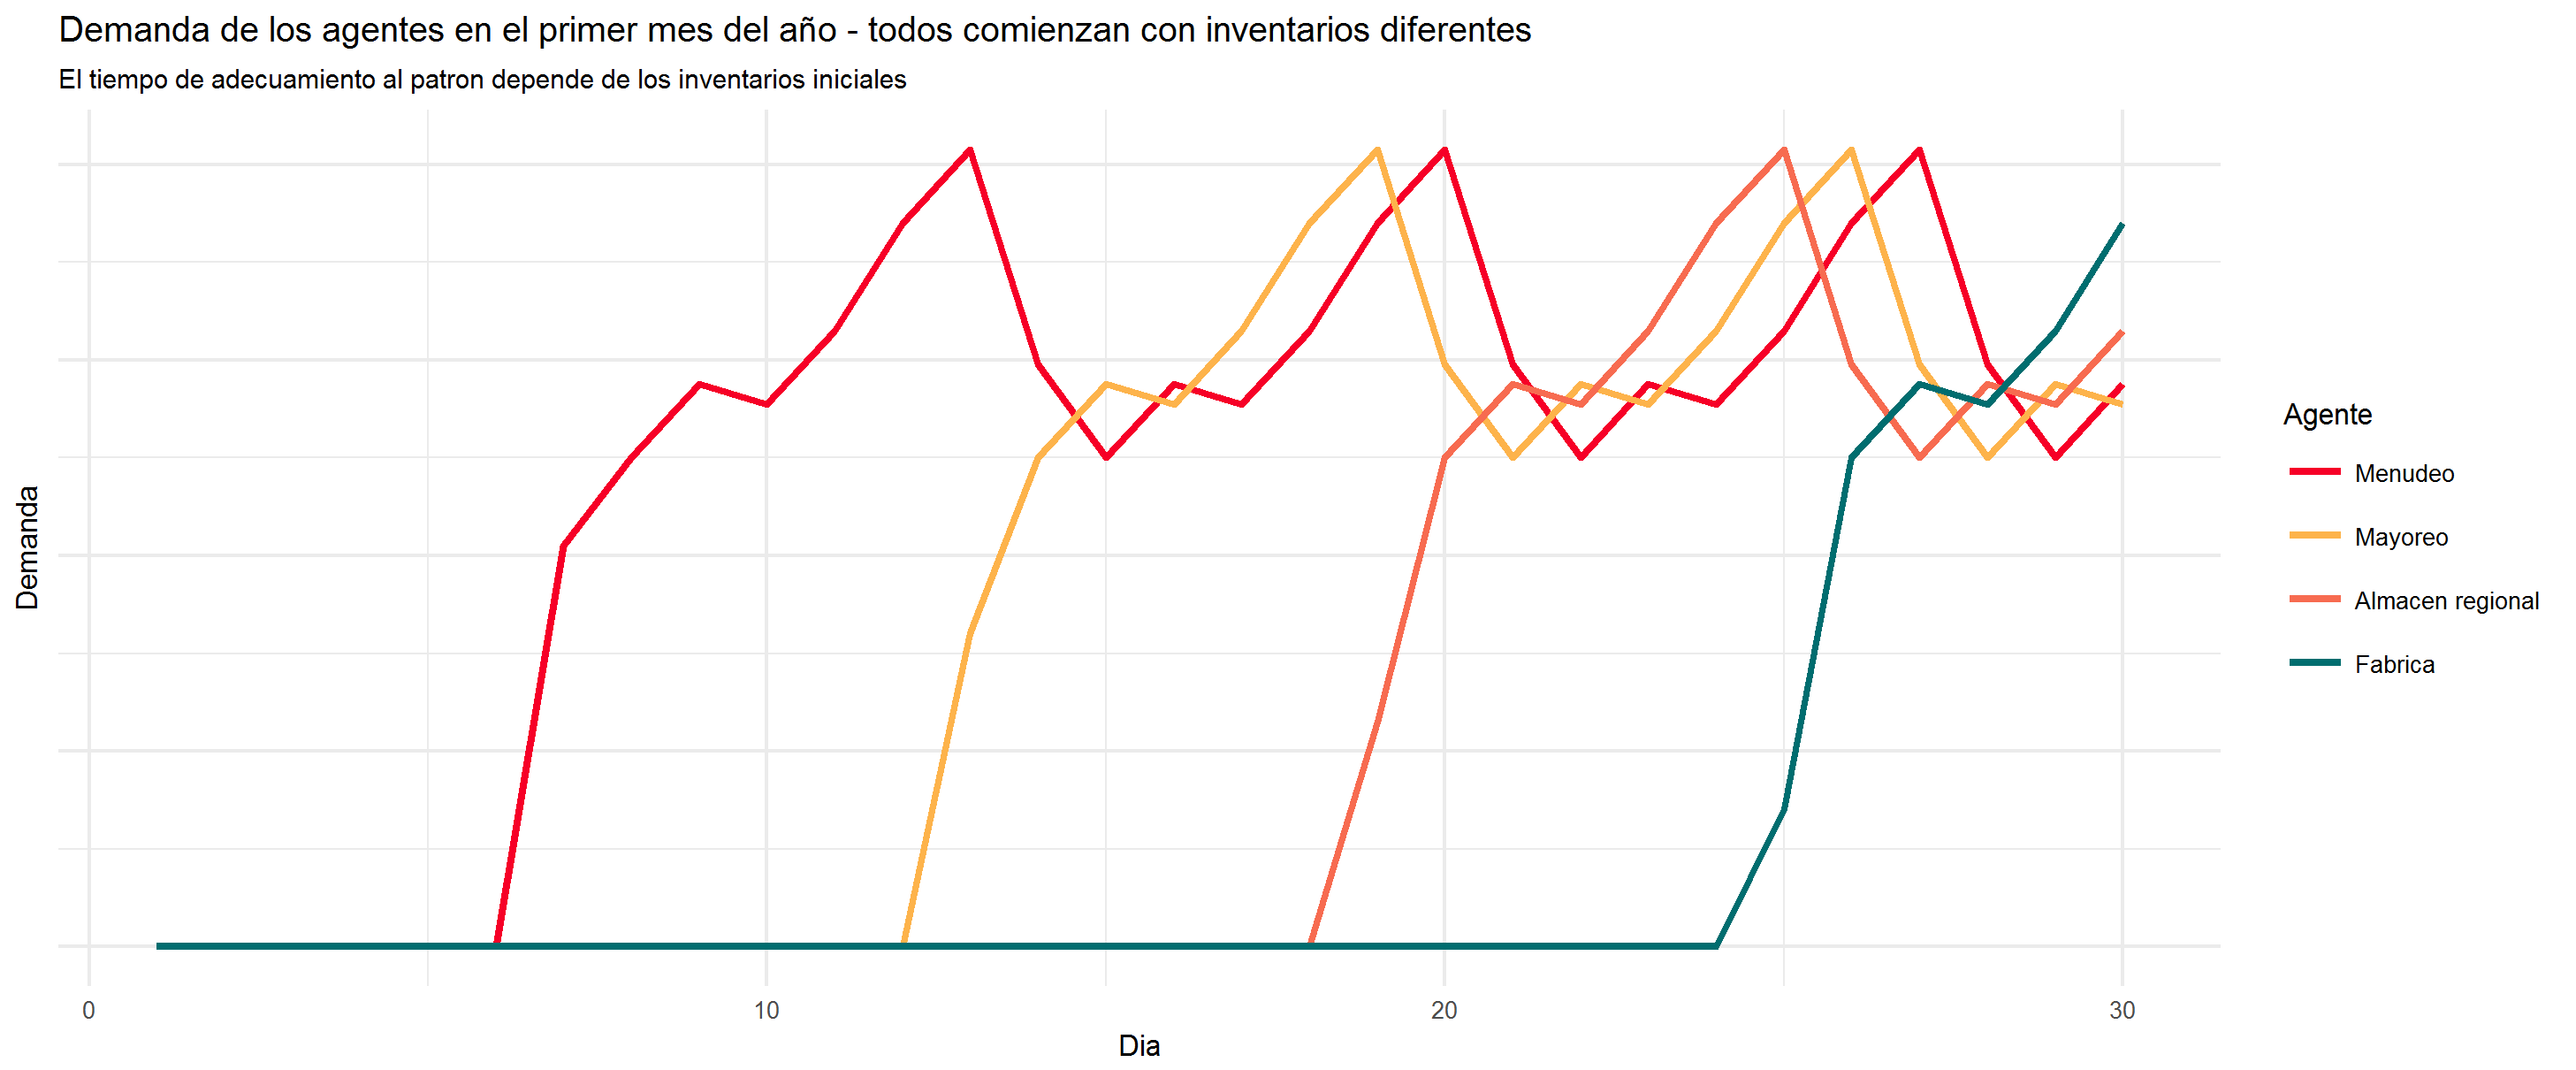
\includegraphics[width=12cm]{tesis_tex/figs/analytic_solution_0_all_45_inv.png}
\centering
\end{figure}

Si la f\'abrica quisiera estimar su demanda para el siguiente a\~no solamente con esta informaci\'on, tendr\'ia que crear un modelo (aunque fuera muy sencillo) para interpolar aquellos d\'ias en los cuales no tuvo informaci\'on. En el caso optimista, usar\'a el mismo patr\'on observado retroactivamente, y tendr\'a una aproximaci\'on relativamente buena. En el caso pesimista, supondr\'a que la demanda del consumidor durante esos d\'ias fue efectivamente cero, y sin duda causar\'a una burbuja de falta de inventario que se propagar\'a hacia abajo en la cadena de suministro. El efecto l\'atigo habr\'a hecho de las suyas.\\



\section{Estacional y aleatoria: m\'as parecido al mundo real}

En el mundo real, ning\'un producto tiene una demanda perfectamente constante. M\'as a\'un, existen una infinidad de productos cuya demanda var\'ia con un patr\'on estacional: por ejemplo, las medicinas antigripales se venden m\'as en invierno. La cerveza (y, en general, las bebidas alcoh\'olicas) tambi\'en siguen este tipo de patrones.\\

En primer lugar, existe un patr\'on semanal bastante esperado: seg\'un \citet{}, se consume m\'as cerveza los fines de semana (ver la figura \ref{weekly_base}). Adem\'as, existe un patr\'on relacionado a las festividades comunes. Seg\'un \citet{}, el consumo de bebidas alcoh\'olicas se duplica en las festividades navide\~nas. \\

\begin{figure}[ht!]
\caption{ }
\label{weekly_base}
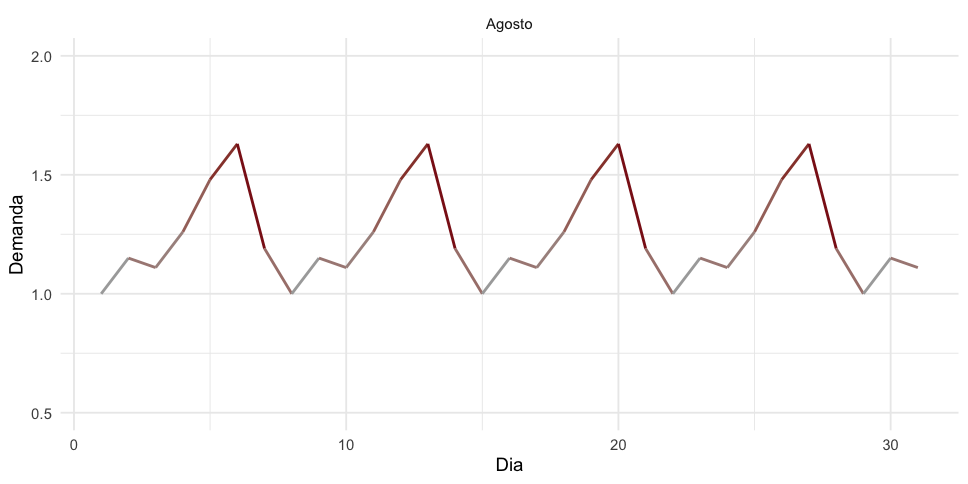
\includegraphics[width=12cm]{monthly_customer_demand_ggplot.png}
\centering
\end{figure}

Para el presente trabajo, combinaremos los dos patrones descritos anteriormente, y a\~nadiremos un peque\~no componente aleatorio que cambiar\'a la demanda cada a\~no. El comportamiento ''base'' de la demanda de puede consultar en la figura \ref{yearly_base}. Un ejemplo del comportamiento perturbado por un poco de aleatoriedad se puede consultar en la figura \ref{yearly_base_noisy}. Sin embargo, cabe mencionar que este es un modelo simple, pues en algunas regiones, podr\'ia tambi\'en existir un patr\'on relacionado al clima, o incluso un alza en la demanda siguiendo temporadas deportivas. \\

\begin{figure}[ht!]
\caption{ }
\label{yearly_base}
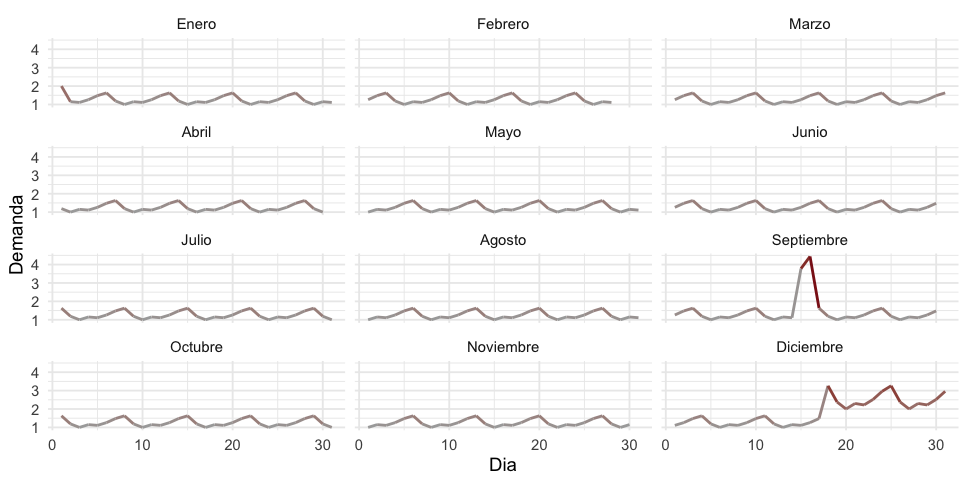
\includegraphics[width=13cm]{monthly_demand_ggplot.png}
\centering
\end{figure}

\begin{figure}[ht!]
\caption{ }
\label{yearly_base_noisy}
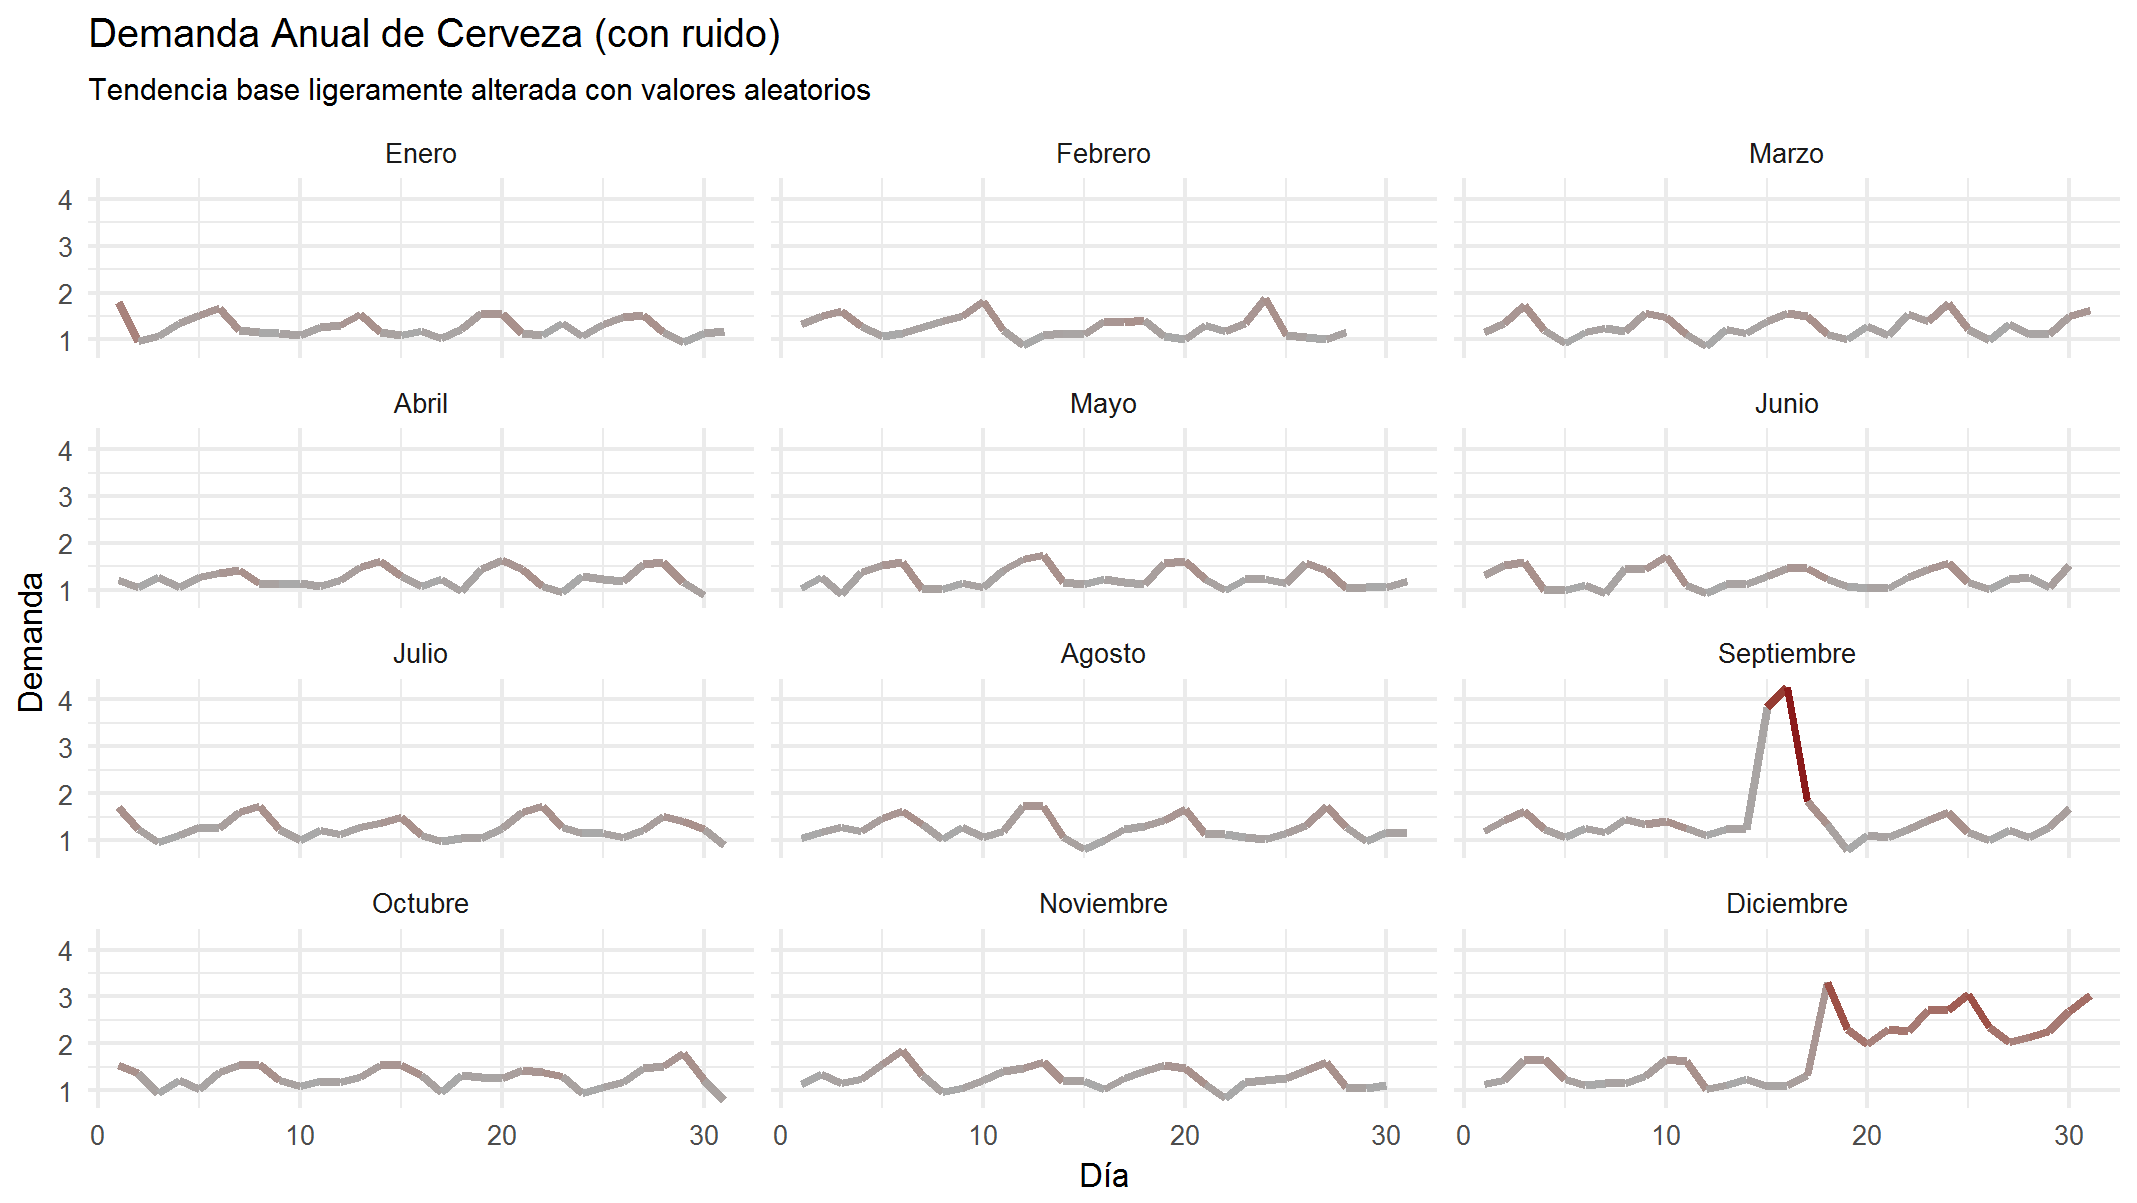
\includegraphics[width=13cm]{monthly_demand_with_noise_ggplot.png}
\centering
\end{figure}

Como el comportamiento var\'ia a lo largo del a\~no y existe un costo por almacenar inventario, cada agente debe prepararse con adecuada anticipaci\'on para los picos de demanda. Adem\'as, el componente aleatorio resulta en la necesidad de conservar inventario de seguridad (en ingl\'es, \textit{safety stock}) para asegurar que la demanda ser\'a cubierta la mayor parte del tiempo.

\section{Q-Learning}

\citet{Chaharsooghi} public\'o ya un acercamiento a este problema usando \textit{Q-learning}, sin embargo la soluci\'on que encuentra implica que los inventarios (al final del d\'ia, despu\'es de las transacciones del d\'ia) se aproximan a cero, consecuencia directa de que los agentes minimizan su costo de inventario. Adem\'as, la demanda del consumidor obedece un patr\'on aleatorio.\\

Sin embargo, ninguna de estas soluciones considera dos factores importantes de la vida real: la temporalidad de la demanda (por ejemplo, para la cerveza la cantidad demandada es mayor durante el fin de semana) y la restricción de temporalidad de producci\'on de materias primas. En el mundo agr\'icola, los campos solamente producen ciertas cosechas en ciertos periodos, y es necesario tener suficiente inventario para cubrir la demanda durante todo el a\~no. En el siguiente cap\'itulo, se presentar\'a este escenario como un nivel extra de complejidad al modelo, limitando la oferta de cebada por parte de los campos.